\chapter{Synthesizing Sound}

The most important feature of a synthesizer is its capability to synthesize sound. Synthesizing sound means to combine two or more (audio) signals to produce a new signal. The many possibilities to synthesize sound waves with variable parameters enable musicians to create an uncountable number of different sounds. A synthesizer can be configured to resemble natural sounds such as that of wind or water waves, can emulate other instruments like pianos, guitars or bass drums and, finally, a synthesizer can also be used to produce entirely new, electronic sounds. However, not all synthesis methods available to the creator of a digital synthesizer are equally suited to the various possible sounds just described. This chapter will examine five popular methods of synthesis --- Additive, Subtractive, Granular, AM and FM synthesis --- while focusing especially on the last technique, which was implemented in C++ for the purpose of this thesis.

\section{Additive Synthesis}

Additive Synthesis was already introduced in Chapter 2 as a method to produce complex waveforms. It involves the summation of a finite set of waveforms that can either be simple sinusoids or complex waves themselves --- such as sawtooth or square waves. As it was already shown, this summation --- formally called a Fourier Series --- can produce a myriad of different waveforms. An example for an Additive Synthesizer is Native Instrument's \emph{Razor}, which lets the user additively synthesize up to 320 partials. Also a simple church organ, whose characteristic sound is produced by the summation of the sounds emitted by its tubes, is an additive synthesizer. In terms of the natural world, Additive Synthesis occurs when any two sound waves meet and combine to produce a new sound.

\section{Subtractive Synthesis}

While Additive Synthesis creates sounds by summing many individual waveforms, Subtractive Synthesis starts out with a complex waveform very rich in harmonics, like a sawtooth wave, and then subtracts or "carves" away parts of that sound by filtering or attenuating selected frequencies. A very prominent example of Subtractive Synthesis is the human voice, which makes use of the larynx to shape air coming from the lungs in order to produce certain phonemes, which eventually make up words, sentences and our ability to communicate.

\section{Granular Synthesis}

A very special form of synthesis is "Granular Synthesis". It produces sound by "splicing" or "concatenating" very short sound samples, referred to as \emph{grains}, "often only a few milliseconds in length". \citebs{12} The synthesized sound can be altered by changing the frequency, amplitude or phase at which certain grains are played. The synthesizer \emph{Malstr{\"o}m} by Propellerhead implements a form of Granular Synthesis (Propellerhead, \url{https://www.propellerheads.se/products/reason/instruments/malstrom/}, accessed 4 January 2015).

\section{Amplitude Modulation Synthesis}

During the discussion of Low Frequency Oscillators (LFOs) in Chapter 3, it was mentioned how a vibrato effect can be achieved by varying the amplitude of a sound using an LFO with a frequency $f$ in the approximate range of $]0;20]$ Hertz. When the frequency of modulation is in the audible range of 20 to 20000 Hertz, this modulation is termed "Amplitude Modulation" (AM). AM produces side-bands in the signal's frequency spectrum and thus changes the sound's timbre. In Amplitude Modulation Synthesis the original signal is termed the "carrier" signal, $c(t)$, and the modulation signal the "modulator", $m(t)$. Equation \ref{eq:am} shows a formula for Amplitude Modulation (Synthesis) with two signals, where $A_{c}$ is the carrier amplitude and $A_{m}$ that of the modulator. Given that already two oscillators can produce a great variety of interesting sounds, Amplitude Modulation Synthesis is a very popular synthesis method found in both the analog as well as the digital realm.

\begin{equation}
  f(t) = (A_{c} + A_{m}\cdot\sin(\omega_{m} t + \phi_{m}))\cdot\sin(\omega_{c} t + \phi_{c})
  \label{eq:am}
\end{equation}

\section{Frequency Modulation Synthesis}

The difference between Amplitude Modulation (AM) and Frequency Modulation (FM) Synthesis is that in the latter, the modulator varies the carrier's frequency as opposed to its amplitude. This produces very complex changes in the carrier's frequency spectrum and introduces a theoretically infinite set of side-bands, which contribute to the characteristic sound and timbre of FM Synthesis. The fact that Frequency Modulation can be used to synthesize audio signals was first discovered by John Chowning, who he described the mathematical principles and practical implications of FM Synthesis in his 1973 paper "The Synthesis of Complex Audio Spectra by Means of Frequency Modulation". In 1974 his employer, Stanford University, licensed his invention to the Yamaha Corporation, a Japanese technology firm, which went on to create the first FM synthesizers, including the very popular DX-7 model. Many digital FM synthesizers, such as Native Instrument's \emph{FM8}, try to emulate the DX-7. (Electronic Music Wiki, \url{http://electronicmusic.wikia.com/wiki/DX7}, accessed 4 January 2015) Equation \ref{eq:fm} gives a full mathematical definition for Frequency Modulation (Synthesis). What Equation \ref{eq:fm} shows is that FM Synthesis works by summing the carrier's instantaneous frequency $\omega_{c}$, the carrier signal being $c(t)$, with the output of the modulator signal $m(t)$, thereby varying the carrier frequency periodically. The degree of frequency variation $\Delta f_{c}$ depends on the modulator's amplitude $A_{m}$. Therefore, $\Delta f_{c} = A_{m}$. Figure \ref{fig:fmlow} shows how frequency modulation effects a signal. Note that this Figure should only show how FM works. It is not a realistic example of FM \emph{Synthesis}, as the modulator frequency is not in the audible range.

\pagebreak

\begin{figure}[]
  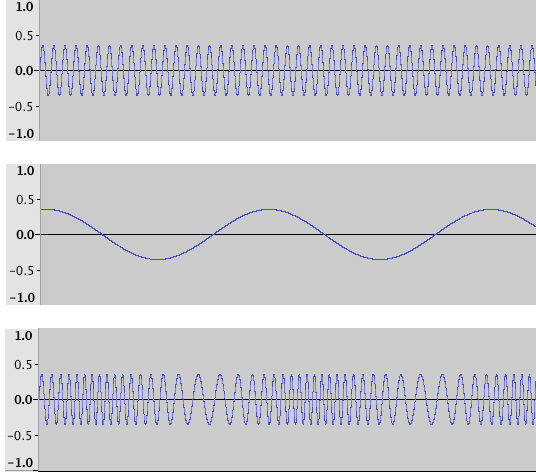
\includegraphics[scale=0.7]{img/fmlow}
  \caption{The first figure shows the carrier signal $c(t)$ with its frequency $f_{c}$ equal to 100 Hz. The signal beneath the carrier is that of the modulator, $m(t)$, which has a frequency $f_{m}$ of 5 Hz. When the modulator amplitude $A_{m}$ is increased to 50 (instead of \textasciitilde{} 0.4, as shown here) and used to modulate the frequency of the carrier, the last signal $f(t)$ is produced. While these figures show how FM works, they are not a good example of FM synthesis, because the modulator frequncy is not in the audible range.}
  \label{fig:fmlow}
\end{figure}

\begin{multicols}{2}
  \begin{equation}
    c(t) = A_{c} \cdot \sin(\omega_{c}t + \phi_{c})
    \end{equation}\break
    \begin{equation}
      m(t) = A_{m} \cdot \sin(\omega_{m}t + \phi_{m})
    \end{equation}
  \end{multicols}

  \begin{equation}
    f(t) = A_{c} \cdot \sin((\omega_{c} + m(t))t + \phi_{c}) = A_{c} \cdot \sin((\omega_{c} + A_{m} \cdot \sin(\omega_{m}t + \phi_{m}))t + \phi_{c})
    \label{eq:fm}
  \end{equation}

  \subsection{Sidebands}

  One of the most noticeable effects of FM Synthesis is that it adds \emph{sidebands} to a carrier signal's frequency spectrum. Sidebands are frequency components higher or lower than the carrier frequency, whose spectral position, amplitude as well as relative spacing depends on two factors: the ratio between the carrier and modulator frequency, referred to as the "C:M ratio", and the index of modulation $\beta$, which in turn depends on the modulator signal's amplitude and frequency.

  \subsection{C:M Ratio}

  The spacing and positions of sidebands on the carrier signal's frequency spectrum depends on the ratio between the frequency of the carrier signal, $C$, and that of the modulator, $M$. This $C:M$ ratio gives insight into a variety of properties of a frequency-modulated sound. Most importantly, when the $C:M$ ratio is known, Equation \ref{eq:sbcm} gives all the relative frequency values of the theoretically infinite set of sidebands. Equation \ref{eq:sbabs} describes how to calculate $\omega_{sb_{n}}$, the angular frequency of the $n$-th sideband, absolutely. What these equations show is that for any given $C:M$ ratio, the sidebands are found at relative frequencies $C + M, C + 2M, C + 3M, ... $ and absolute frequencies %
  $\omega_{c} + \omega_{m}, \omega_{c} + 2 \omega_{m},\omega_{c} + 3 \omega_{m}, ...$ Hertz.

  \begin{equation}
    \omega_{{sb}_{n}} = C \pm n \cdot M, \text{where } n \in [0;\infty[
    \label{eq:sbcm}
  \end{equation}

  \begin{equation}
    \omega_{{sb}_{n}} = \omega_{c} \pm n \cdot \omega_{m}, \text{where } n \in [0;\infty[
    \label{eq:sbabs}
  \end{equation}

  \noindent When examining these two equations one may notice that there also exist sidebands with negative frequencies, found relatively at $C - M, C - 2M, C - 3M$ and so on. Simply put, a signal with a negative frequency is equal to its positive-frequency counterpart but with inverted amplitude, which can also be seen as a 180\degree{} or $\pi$ radian phase-shift (\url{http://www.sfu.ca/~truax/fmtut.html}, accessed 30 December 2014). Equation \ref{eq:negfreq} defines this formally. What this also means is that if there is a sideband at a frequency $f$ and another sideband at $-f$ Hertz, these two sidebands will phase-cancel completely if their amplitudes are the same. If not, the positive side-band will be reduced in amplitude proportionally. Consequently, it may happen that also the original carrier frequency is reduced in amplitude, for example at a $C:M$ ratio of 1:2, as the first "lower" sideband, meaning with a lower frequency than the carrier, is at $C - M = C - 2C = -C$ Hertz.

  \begin{equation}
    A \cdot \sin(-\omega t + \phi) = -A \cdot \sin(\omega t + \phi) = A \cdot \sin(\omega t + \phi - \pi)
    \label{eq:negfreq}
  \end{equation}

  \noindent Figure \ref{fig:sb} shows the frequency spectrum of a carrier signal with a frequency $f_{c}$\footnote{Not to be confused with the cutoff frequency in the context of filters, which is also denoted by $f_{c}$} of 200 Hz, modulated by a modulator signal with its frequency $f_{m}$ equal to 100 Hz. The carrier frequency is seen on the spectrum as the peak at 200 Hz. The other peaks are the sidebands. Because the $C:M$ ratio here is $2:1$, the first two lower sidebands are found at relative positions $C-M=2-1=1$ and $C-2M=2-2=0$, relative position $2$ being the carrier. The first two upper sidebands have absolute frequency values of $\omega_{c} + \omega_{m} = 200 + 100 = 300$ and %
  $\omega_{c} +2\cdot\omega_{m} = 200 + 200 = 400$ Hertz.\\

  \begin{figure}[]
    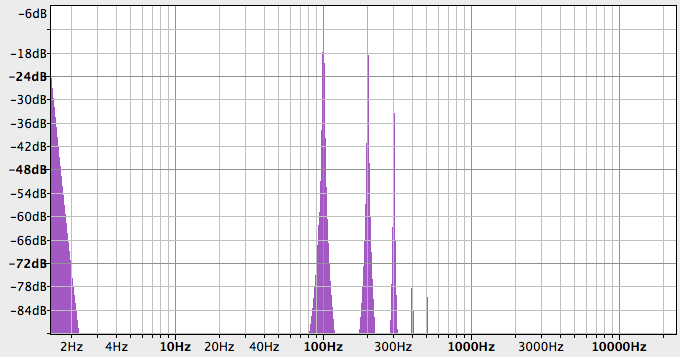
\includegraphics[scale=0.5]{img/sb}
    \caption{The frequency spectrum of a $C:M$ ratio of $2:1$, where carrier frequency $f_{c}$ is 200 and the modulator frequency $f_{m}$ 100 Hertz.}
    \label{fig:sb}
  \end{figure}

  \pagebreak

  \noindent The $C:M$ ratio can also help to understand how a frequency-modulated signal will sound. For example, a ratio of $1:2$ will sound similar to a square wave, since the harmonic series produced by this ratio will have sidebands at $3C, 5C, 7C$ etc., so, all odd partials. On the other hand, a $C:M$ ratio of $1:1$ will cause the resulting sound to resemble a sawtooth wave, as the sidebands are positoned at $2C, 3C, 4C, ...$, which fits the requirement of a sawtooth wave to be composed of \emph{all} partials. Figure \ref{fig:fmsaw} shows how a ratio of $1:1$ causes the signal to look a lot like a sawtooth wave with two partials. Even though this waveform includes all partials, it does not look like a perfect sawtooth wave, as it would if it had been created by additive synthesis. The reason why is that the amplitude of each partial is not the inverse of the partial number, but some other value. The same applies to square waves.\\

  \begin{figure}[]
    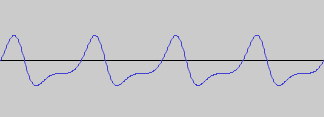
\includegraphics[scale=0.7]{img/fmsaw}
    \caption{A sound wave produced by FM Synthesis that resembles a sawtooth wave with two partials visually as well as acoustically. The reason why is that the $C:M$ ratio was $1:1$ in this case, causing sidebands to be a perfect harmonic series.}
    \label{fig:fmsaw}
  \end{figure}

  \noindent There is also a way to find out if a $C:M$ ratio will result in a harmonic series or in an inharmonic series. To re-cap, a harmonic \emph{sideband} is an integer multiple of the carrier frequency while an inharmonic sideband is not. A harmonic \emph{series} with a harmonic \emph{ratio}, such as $1:2$, includes only harmonic sidebands and has the carrier frequency as the fundamental pitch, while an inharmonic series with an inharmonic ratio, e.g. $2:5$, includes one or more inharmonic sidebands. For a general procedure to determine the \emph{harmonicity} of a $C:M$ ratio, the ratio first has to be converted to \emph{Normal Form}. In Normal Form, "$M$ must be greater or equal to twice $C$ or else be the ratio $1:1$". To \emph{normalize} a ratio that is not in Normal Form, the operation $C = | C - M |$ is performed until the Normal Form criterion is met. For example, to normalize a ratio of $5:2$: $5 - 2 = 3 \rightarrow 3 - 2 = 1 \Rightarrow 1:2$. Once a ratio has been brought into Normal Form, the rule to determine if a ratio will result in a harmonic series is the following: "harmonic [Normal Form] ratios are always of the form $1:N$, and inharmonic ones [are not]". Therefore, normalized ratios like
  $1:2, 1:5, 1:10$ are inharmonic, while examples for inharmonic ratios are $2:9, 3:8 \text{ or } 4:9$.
  (\url{http://www.sfu.ca/~truax/fmtut.html}, accessed 30 December 2014)

  \subsection{Index of Modulation}

  Theoretically, Frequency Modulation Synthesis produces an infinite number of sidebands. However, sidebands reach inaudible levels very quickly, making the series practically finite. In general, the amplitude of individual sidebands depends on the "index of modulation" and the Bessel Function values that result from it. A definition for the index of modulation, denoted by $\beta$, is given in Equation \ref{eq:beta1}. Because the variation in carrier frequency, $\Delta f_{c}$, depends directly on the amplitude of the modulator, Equation \ref{eq:beta1} can be re-written as Equation \ref{eq:beta2}.

  \begin{multicols}{2}

    \begin{equation}
      \beta = \frac{\Delta f_{c}}{f_{m}}
      \label{eq:beta1}
    \end{equation}

    \begin{equation}
      \beta = \frac{\Delta f_{c}}{f_{m}} = \frac{A_{m}}{f_{m}}
      \label{eq:beta2}
    \end{equation}

  \end{multicols}

  \noindent The index of modulation can be used to determine the amplitude of individual sidebands, if input into the Bessel Function, shown in Equation \ref{eq:bessel}, where $n$ is the sideband to calculate the amplitude for. Table \ref{tb:bessel} shows amplitude values for the $n$-th sideband, given an index of modulation $\beta$. These values were derived from the Bessel Function. Only  values above 0.01 are shown.

  \begin{equation}
    J(n,\beta) = \sum_{k=0}^{\infty} \frac{(-1)^{k} \cdot (\frac{\beta}{2})^{n+2k}}{(n+k)! \cdot k!}
    \label{eq:bessel}
  \end{equation}

  \begin{table}[h!]

    \begin{tabular}{*{10}{|l}|}
      \hline
      \rowcolor[gray]{0.8}
      & \multicolumn{9}{c|}{Sideband} \\
      \cline{2-10}
      \cellcolor[gray]{0.8} \multirow{-2}{*}{$\beta$} & Carrier & 1 & 2 & 3 & 4 & 5 & 6 & 7 & 8 \\
      \hline
      0 & 1 &&&&&&&& \\
      \hline
      0.25 & 0.98	& 0.12 &&&&&&& \\
      \hline
      0.5 & 0.94 & 0.24	& 0.03 &&&&&& \\
      \hline
      1.0 & 0.77 & 0.44 & 0.11 & 0.02 &&&&& \\
      \hline
      1.5 & 0.51 & 0.56	& 0.23 & 0.06	& 0.01 &&&& \\
      \hline
      2.0 & 0.22 & 0.58	& 0.35 & 0.13	& 0.03 &&&&\\
      \hline
      3.0 & -0.26 & 0.34 & 0.49 & 0.31 & 0.13	& 0.04 & 0.01 && \\
      \hline
      4.0 & -0.40 & -0.07 & 0.36 & 0.43	& 0.28 & 0.13 & 0.05 & 0.02 & \\
      \hline
      5.0 & -0.18 & - 0.33 & 0.05 & 0.36	& 0.39 & 0.26 & 0.13 & 0.05	& 0.02 \\
      \hline
    \end{tabular}

    \caption{}

    \label{tb:bessel}

  \end{table}

  \noindent Another useful property of the index of modulation is that it can be used to provide an intuitive interface to the user of a synthesizer. Instead of having to control the absolute modulator amplitude, which can be rather hard to tune, some synthesizers provide the user with a range of $[0;10]$ to control $\beta$. Behind the scenes, the modulator amplitude $A_{m}$ is then calculated as $\beta \cdot f_{m}$, where $f_{m}$ is the modulator frequency. Moreover, also the modulator frequency is often not shown absolutely in a synthesizer's interface, but relative to the carrier's frequency, e.g. at a ratio of 2 times the carrier frequency $f_{c}$ (the $C:M$ ratio is therefore always $1:M$). (JCPedroza, \url{http://sound.stackexchange.com/questions/31709/what-is-the-level-of-frequency-modulation-of-many-synthesizers}, accessed 3 January 2015)

  \subsection{Bandwidth}

  The bandwidth of a signal describes the range of frequencies that signal occupies on the frequency spectrum. The bandwidth of a frequency-modulated signal is theoretically infinite. However, it was already shown that the amplitude values of a carrier's sidebands quickly become inaudible and thus negligible. A rule of thumb for calculating the bandwidth $B$ of an FM signal is the so-called "Carson Bandwidth Rule", given in Equation \ref{eq:bw}.

  \begin{equation}
    B \approx 2(\Delta f_{c} + f_{m}) = 2(A_{m} + f_{m}) = 2f_{m}(1 + \beta)
    \label{eq:bw}
  \end{equation}

  \subsection{Algorithms and Operators}

  When speaking of FM Synthesis, it is common to refer to oscillators as "operators". This naming convention stems from the Yamaha DX-7 series. So far, FM Synthesis was only discussed for two operators, a carrier and a modulator. However, it is entirely possible to perform FM Synthesis with more than two operators, by modulating any number of operators either in series, or in parallel. When three operators $A$, $B$ and $C$ are connected in series, $A$ modulates $B$, which in turn modulates $C$. If $A$ and $B$ are connected in parallel, but in series with $C$, $C$ is first modulated by $A$ and then by $B$. The same result is achieved if the sum of signals $A$ and $B$ is used to modulate $C$. In general, a configuration of operators is referred to as an "algorithm". The number of possible algorithms increases with an increasing number of operators. In the synthesizer created for this thesis, four operators $A$, $B$, $C$ and $D$ are used. The possible algorithms for these four operators are shown in Figure \ref{fig:fmalgs}.

  \begin{figure}[p!]
    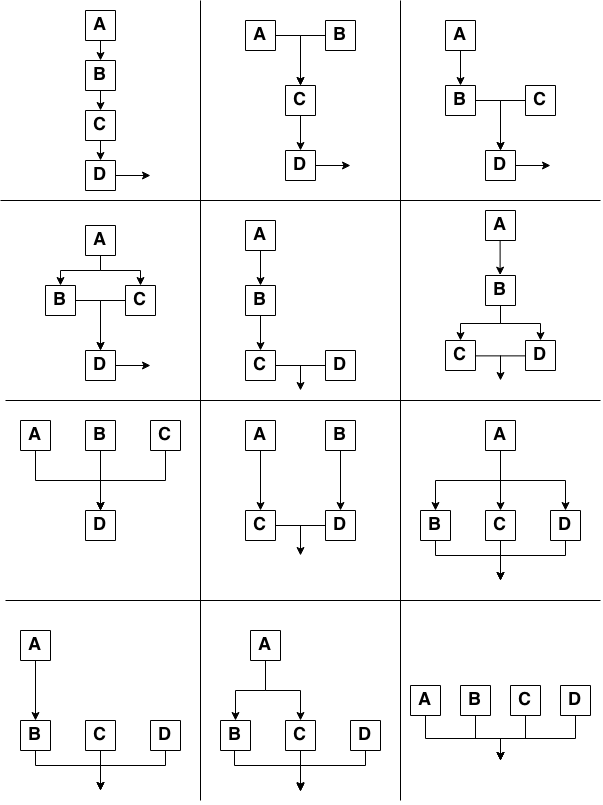
\includegraphics[scale=0.75]{img/fmalgs}
    \caption{Signal flows for FM Synthesis algorithms with four operators, $A$, $B$, $C$ and $D$. A direct connection between two operators means modulation of the bottom operator by the top operator. Signals of operators positioned side-by-side are summed.}
    \label{fig:fmalgs}
  \end{figure}

  \subsection{Implementation}

  The \texttt{Operator} class implements an FM operator and inherits from the \texttt{Oscillator} class. Its frequency is modulated by adding an offset to its Wavetable index increment, proportional to the frequency variation caused by the modulator. Table \ref{code:operator} shows how this offset is calculated and added to the Wavetable index whenever the Operator is updated. Listing \ref{code:fm} shows how the \texttt{FM} class, which takes pointers to four Operators, implements the various algorithms shown in Figure \ref{fig:fmalgs}.

  \begin{table}[hb!]
    \code{operator.cpp}
    \caption{Two member functions from the \texttt{Operator} class that show how the frequency of an \texttt{Operator} object can be modulated.}
    \label{code:operator}
  \end{table}
